\chapter{Probabilistically}

\section{Probability that SS remains at home}

Finding the probability of SS remaining at home after taking $2n$ steps is the same as finding the probability of heads showing up as many times as tails after $2n$ flips or vice-versa. This is because for SS to remain at the initial point after walking randomly, the distance traveled in each direction must be the same so they cancel out. Since the step size is the same for both directions, the number of steps taken in each direction must also be the same as well.

Since SS is walking $2n$ steps each day, the number of steps he is taking each direction must be $n$. Thus, we can define the probability of him remaining at home after his random walks can simply be found using binomial distribution.

\begin{equation}
\begin{aligned}
	Pr[\#H = n]
		&=\binom{2n}{n}\left(\frac{1}{2}\right)^n\left(\frac{1}{2}\right)^n \\
		&=\binom{2n}{n}\left(\frac{1}{2}\right)^{2n} \equiv \frac{(2n)!}{(n!)^2 \cdot 2^{2n}}
\end{aligned}
\end{equation}

\begin{figure}[h]
	\centering
	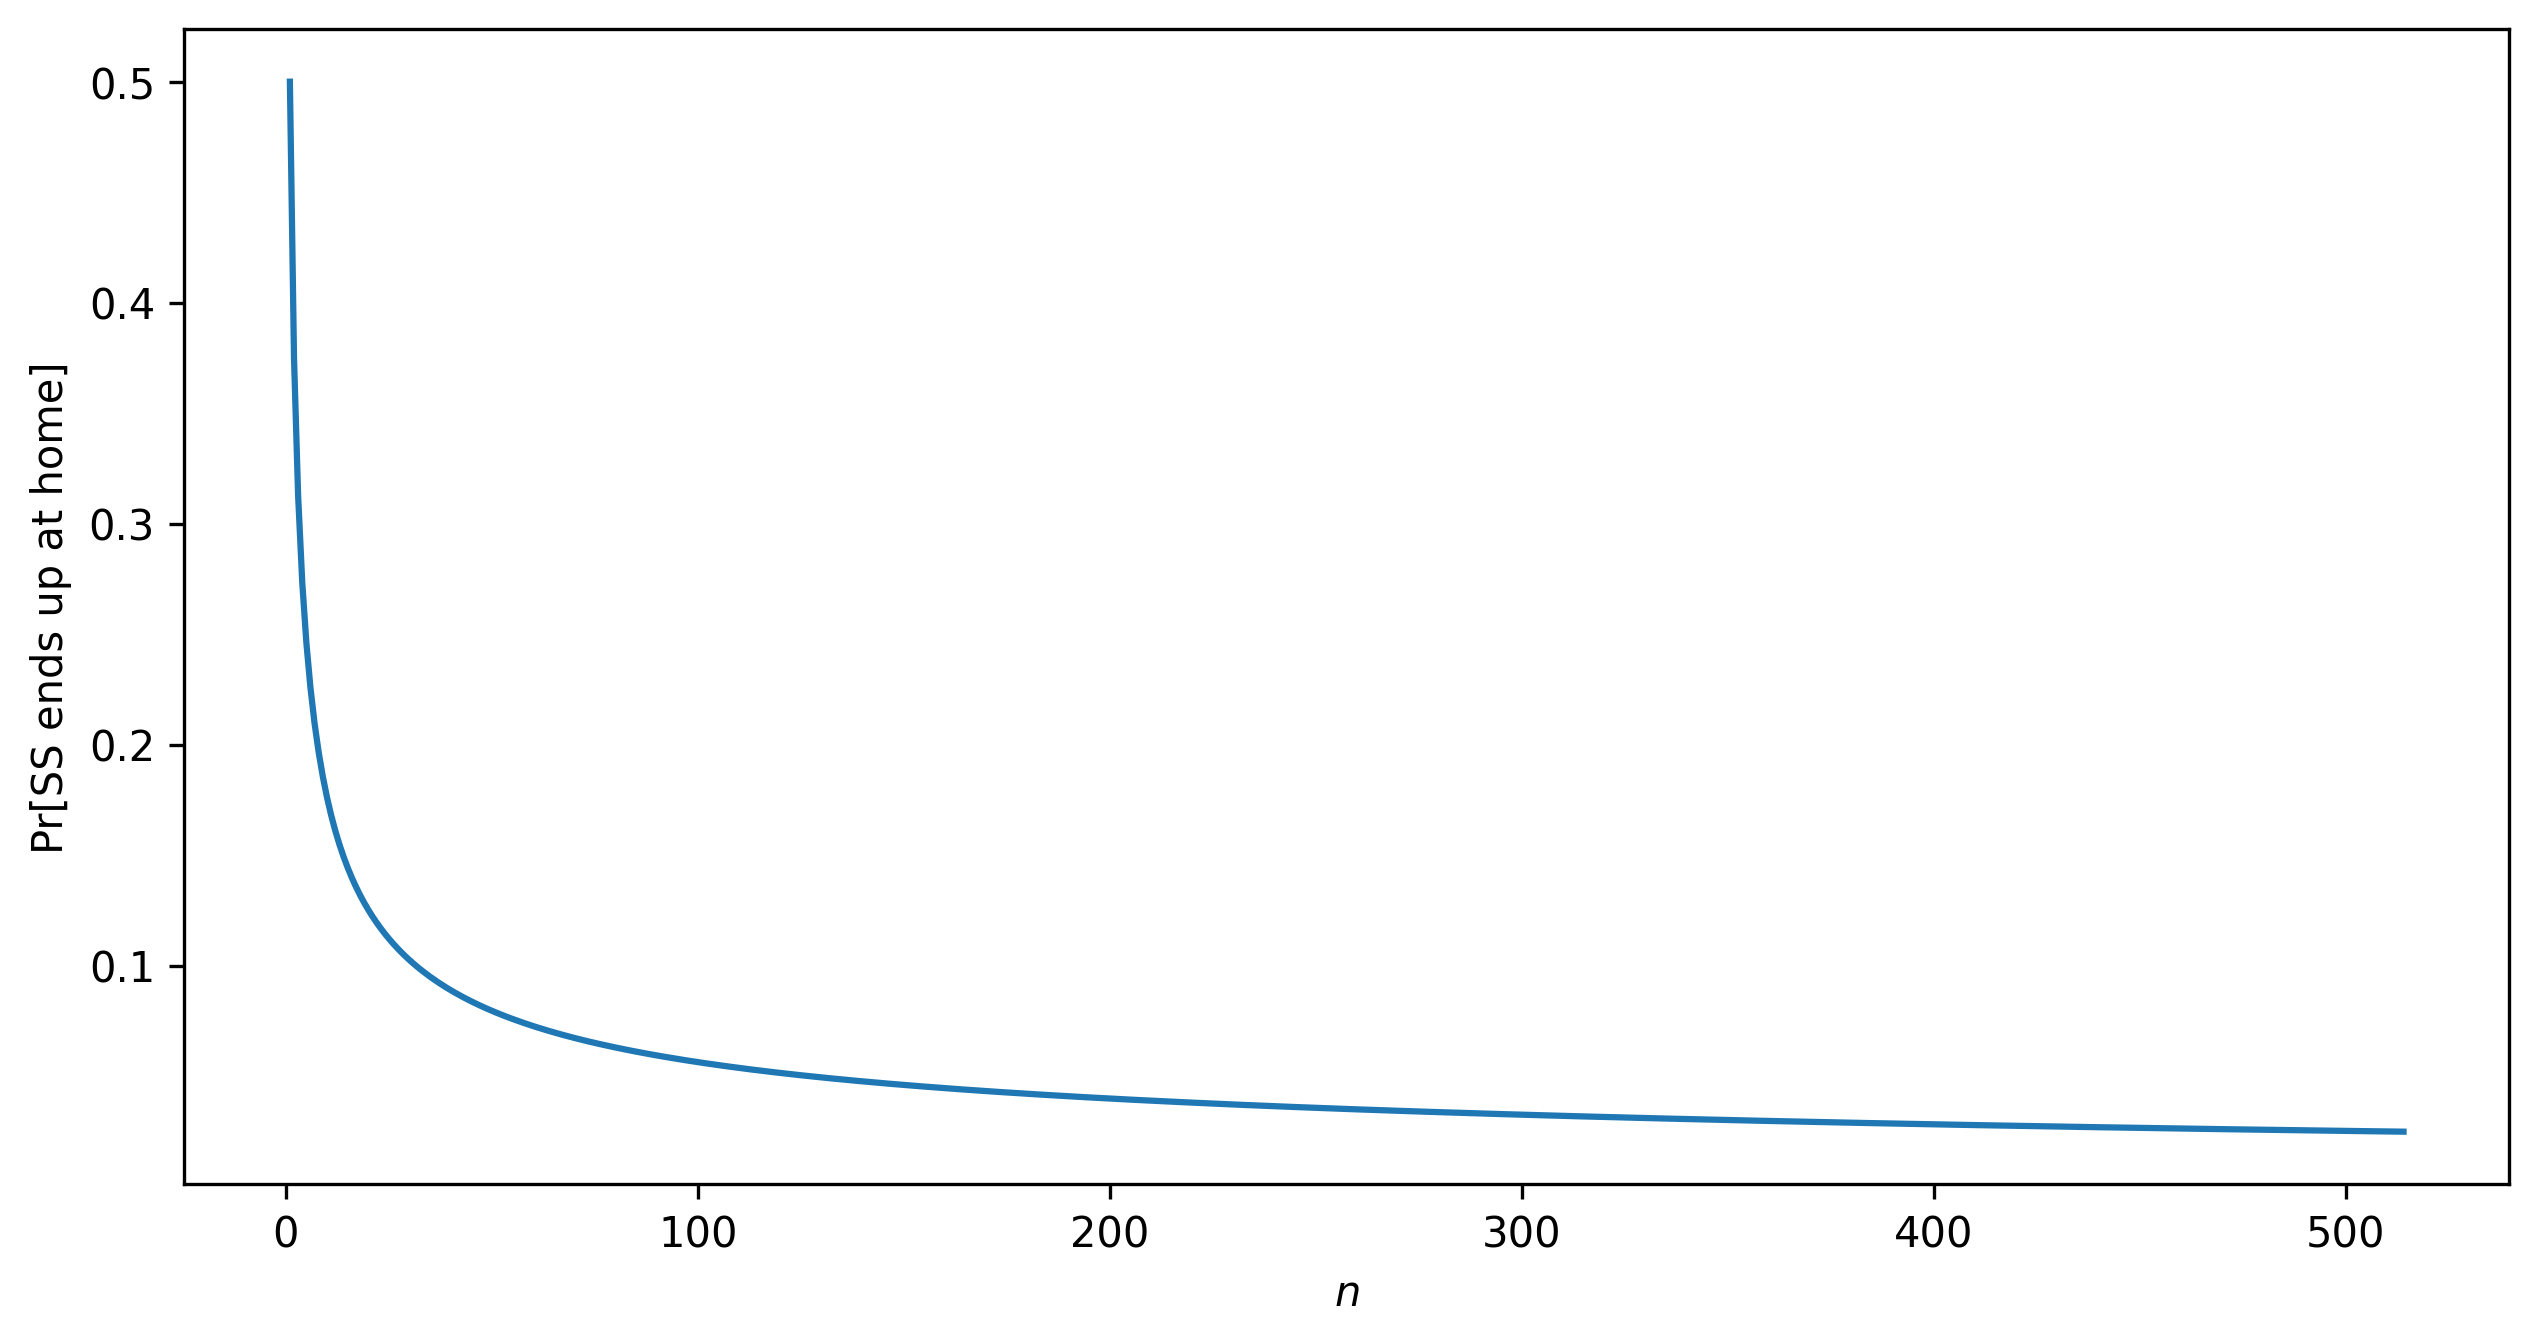
\includegraphics[width=0.8\textwidth]{graphics/02-endsathome.png}
	\caption{Trend as $n$ increases}
\end{figure}

\section{Expected number of times SS arrives home}

While there is a closed form out there for calculating the expected number of times SS returns home in the $2n$ steps,
we will use Monte Carlo simulation to give us some sample and try to fit a line to it.

\begin{figure}[h]
	\centering
	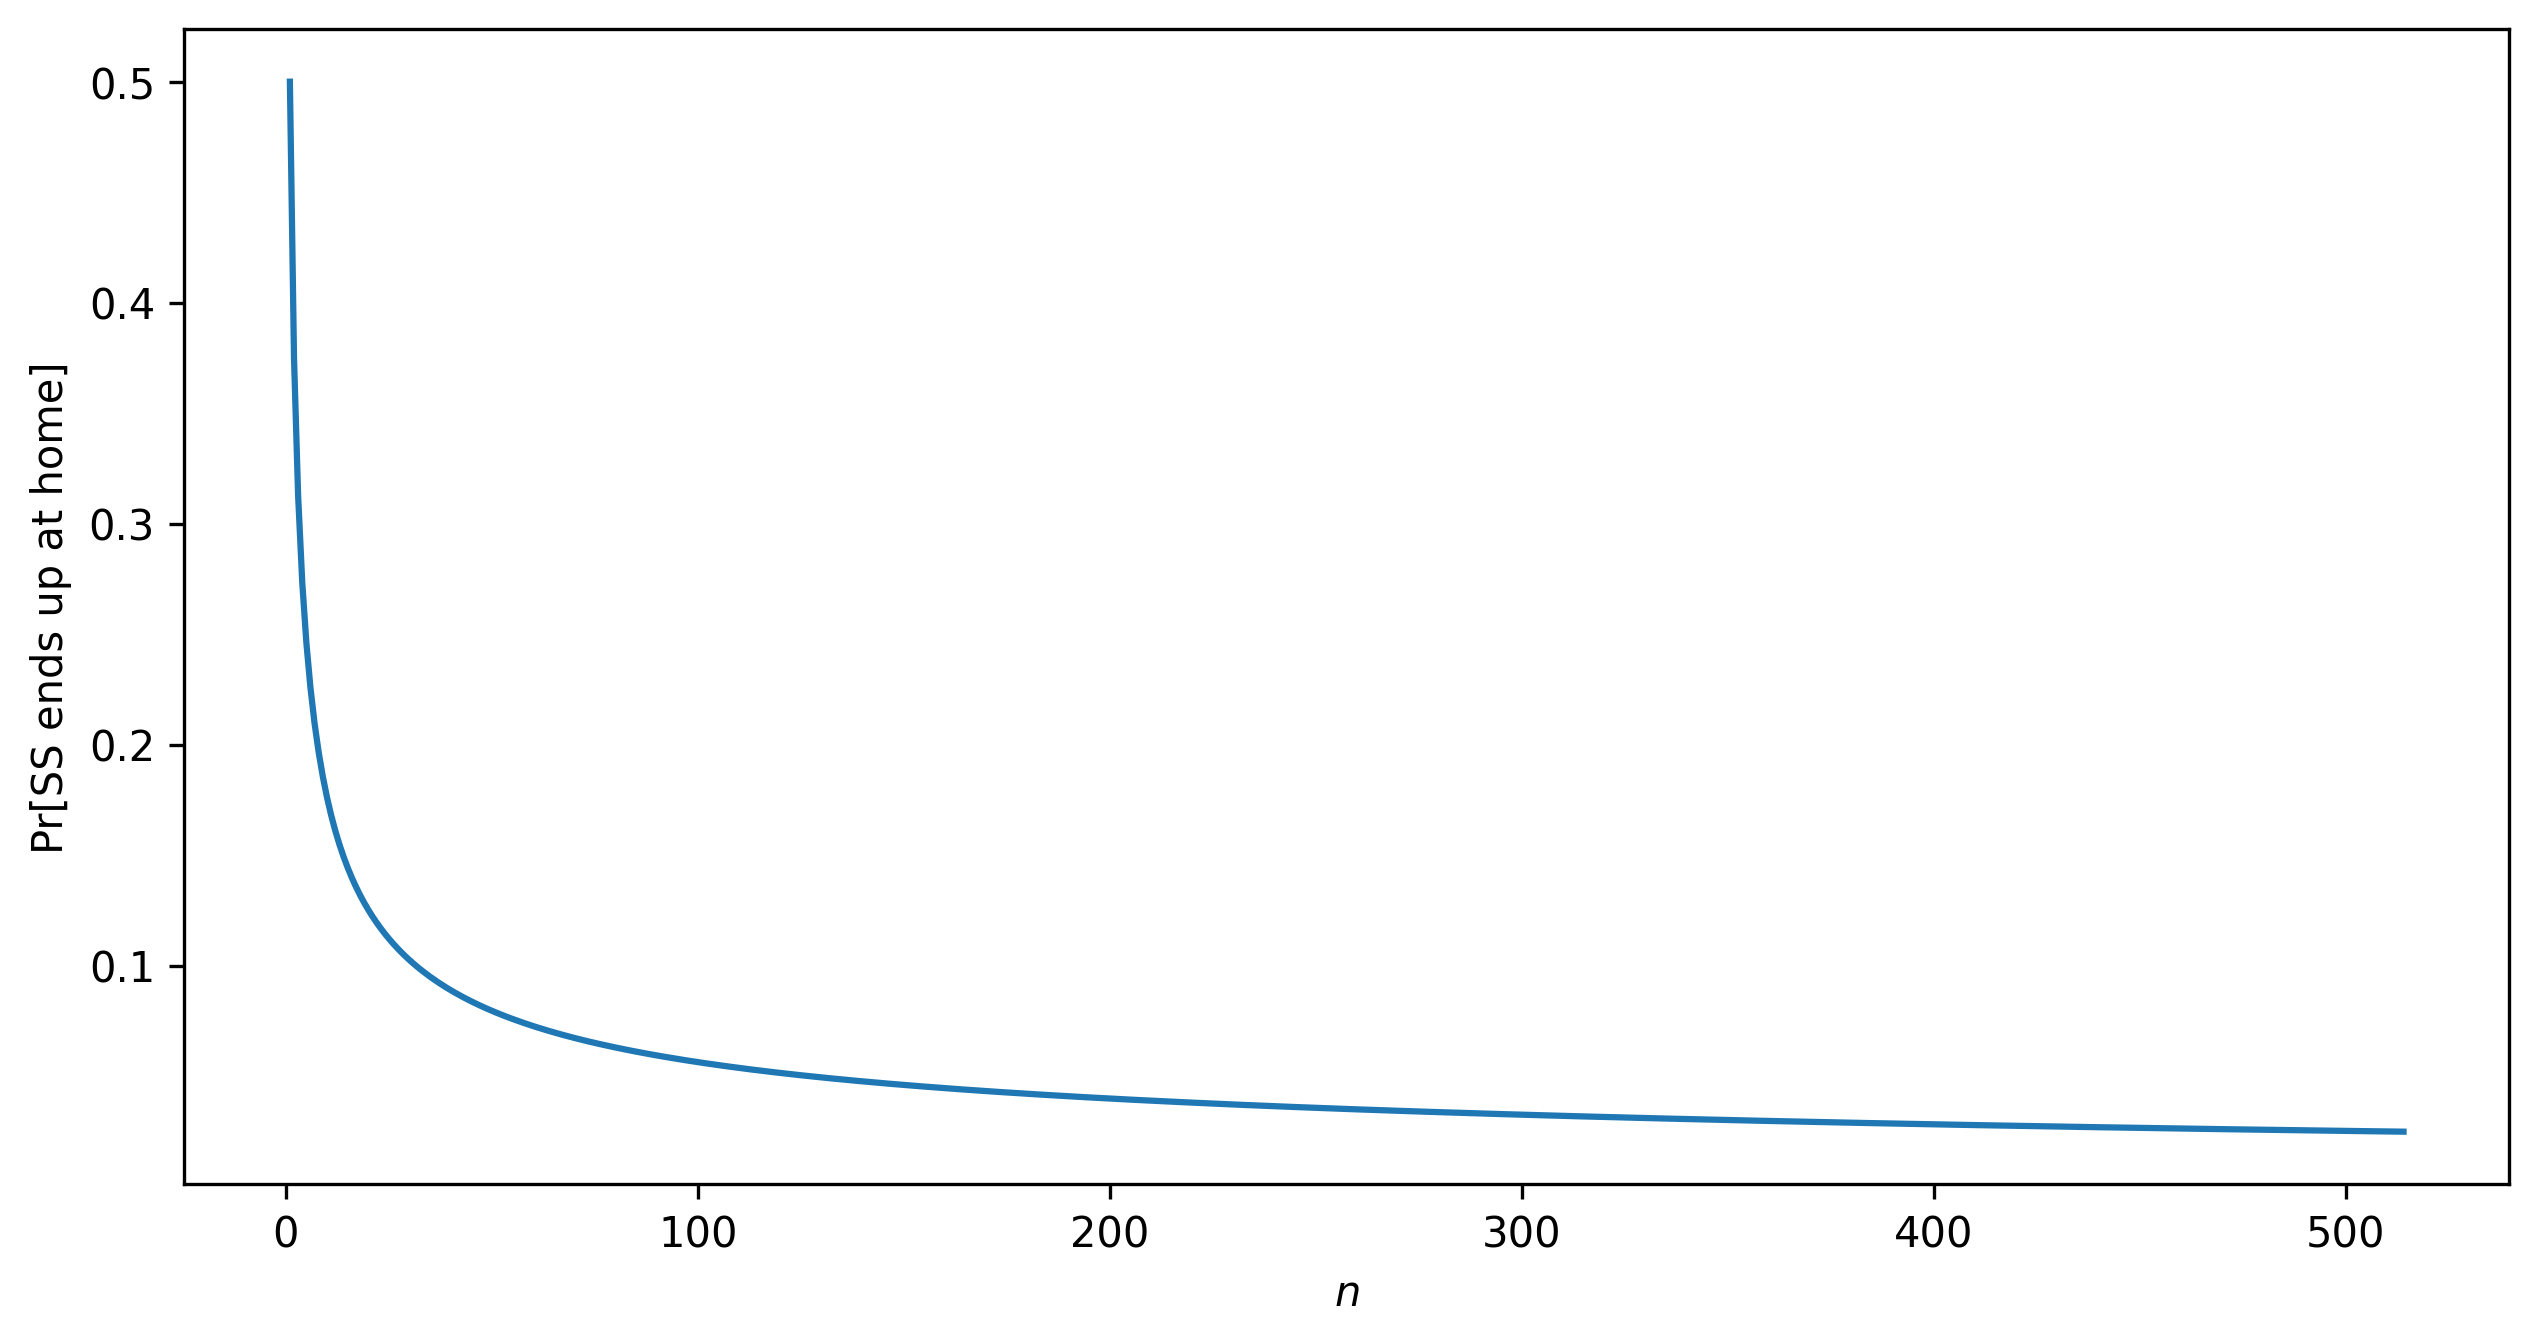
\includegraphics[width=0.8\textwidth]{graphics/02-endsathome.png}
	\caption{Average number of times SS passes his home}
\end{figure}
